\chapter{Data Quality and Initial Exploratory Assessment}

Before conducting the performance analysis, the advertising campaign dataset was assessed to ensure that it was suitable for business decision-making. A comprehensive data quality assessment was performed, including verification of data types, duplicate records, missing values, logical consistency, and potential outliers. 

The complete details of these procedures are provided in Appendix~\ref{appendix:data_quality}.

\subsection{Data Cleaning Summary}

The data cleaning process consist of:

\begin{itemize}
	\item Verified variable data types
	
	\item Checked duplicate observations
	
	\item Removing observations(20 datapoints) with missing revenue.
	
	\item Retaining structurally missing Video Completion Rate values.
	
	\item Retaining valid view-through conversions.
	
	\item Removing observations(47 datapoints) with 0 clicks,impressions and purchases with non-zero purchase. 
	
	\item Addressed severe \texttt{Spend} outliers.
	
	
	
	
\end{itemize}

Overall, the dataset was determined to be sufficiently complete and reliable for subsequent analysis.

\subsection{Challenge}


The primary business challenges include:

\begin{itemize}
	\item Overall ROAS is substantially below the target value.
	\item Campaign performance varies considerably across advertising platforms, creative types, and product categories.
	\item Weekly ROAS has shown a declining trend, indicating decreasing advertising efficiency.
	\item Regional performance differences remain unclear.
	\item The impact of competitive events on campaign performance is uncertain.
	\item The effectiveness of different creative types and audience segments has not yet been established.
	\item Advertising spend must be reduced in underperforming areas while maintaining revenue growth.
\end{itemize}

\subsection{Performance Metrics}

We need numbers to evaluate campaign effectiveness. In that regard, four standard digital marketing performance metrics were considered.

\begin{table}[H]
	\centering
	\begin{tabular}{ll}
		\toprule
		Metric & Formula\\
		\midrule
		CTR & Clicks / Impressions\\
		CPC & Spend / Clicks\\
		CVR & Purchases / Clicks\\
		ROAS & Revenue / Spend\\
		\bottomrule
	\end{tabular}
	\caption{Calculated performance metrics.}
\end{table}

These metrics provide standardized measures of audience engagement, advertising efficiency, conversion effectiveness, and financial return.

\section{Initial Exploratory Assessment}

\subsection{Business Overview}

Following data cleaning, the overall Return on Advertising Spend (ROAS) is 0.96, which is below the company's target of 1.20. This indicates that the current advertising strategy is not generating sufficient revenue relative to advertising expenditure. Performance also varies across campaigns, platforms, creative types, product categories, and target audiences, suggesting opportunities to improve budget allocation and campaign effectiveness.

Since improving ROAS is the primary business objective, the subsequent analysis focuses on identifying the factors associated with both high- and low-performing advertising campaigns.

\subsection{Key Performance Metrics}

To evaluate advertising performance, the following baseline metrics were selected.

\begin{table}[H]
	\centering
	\begin{tabular}{lp{10cm}}
		\toprule
		Metric & Business Relevance\\
		\midrule
		Spend & Measures advertising investment and budget allocation.\\
		
		Revenue & Measures the financial return generated by advertising activities.\\
		
		ROAS & Primary indicator of advertising efficiency and campaign profitability.\\
		
		CTR & Measures audience engagement with advertisements.\\
		
		CPC & Measures the cost required to generate user engagement.\\
		
		CVR & Measures the effectiveness of converting engaged users into customers.\\
		
		\bottomrule
	\end{tabular}
	\caption{Baseline performance metrics used throughout the analysis.}
\end{table}

Together, these metrics provide a comprehensive view of advertising performance, covering investment, engagement, conversion, and financial return.

\subsection{Preliminary Insights}
I created a power BI dashboard(file is inside github repository) to summarize the ROAS to gives us a main idea of the campaign ad ROAS across different categorical variables.

\begin{figure}[h]
	\centering
	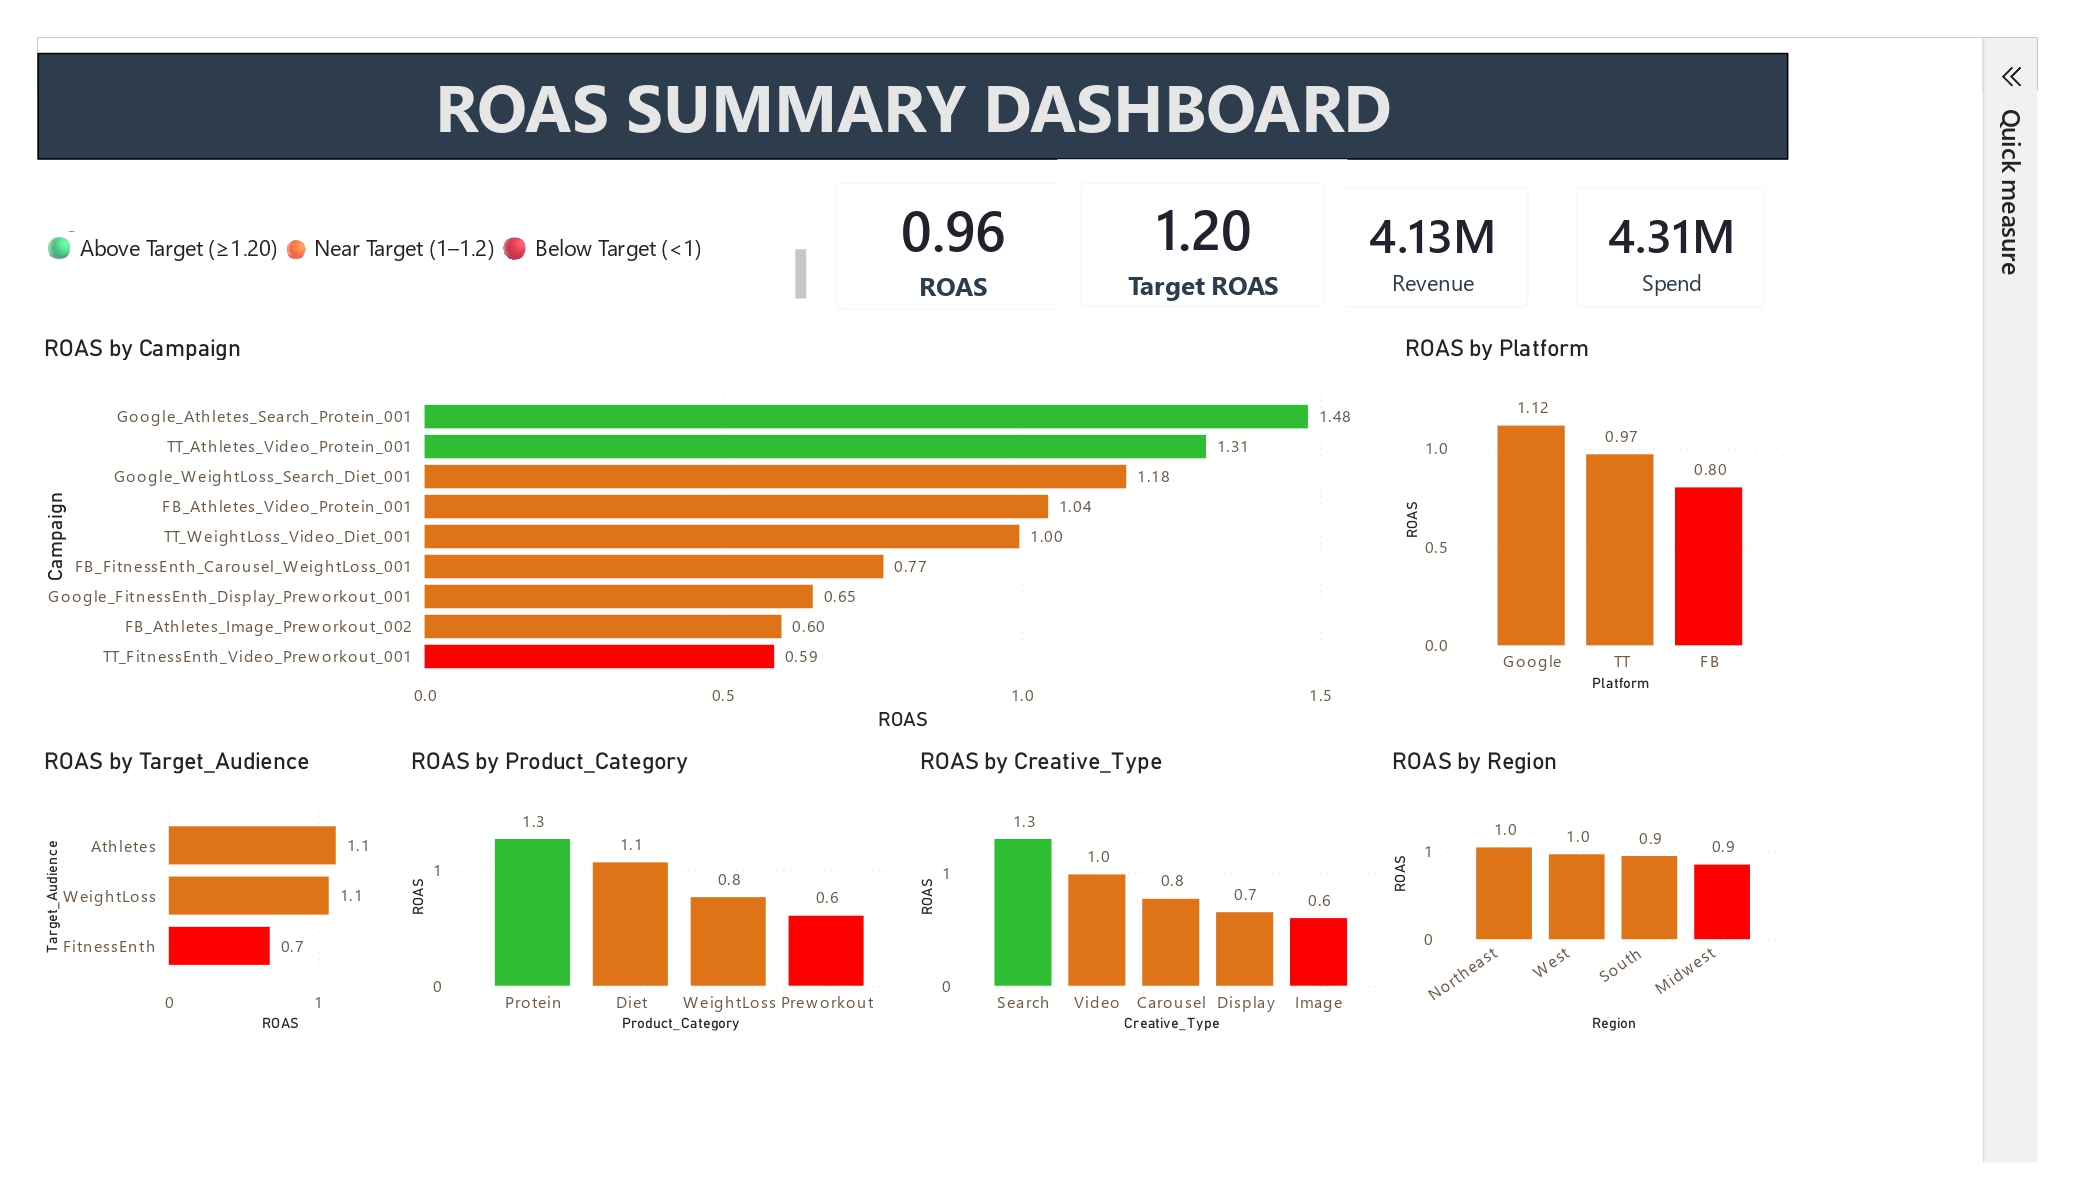
\includegraphics[width=1\textwidth]{images/roas_summary.jpg}
	\caption{ROAS Dashboard Summary}
	\label{fig:roas_summary}
\end{figure}

The executive dashboard provides an initial overview of advertising performance prior to detailed analysis. Several observations can be made:

\begin{itemize}
	
	\item Overall ROAS (0.96) remains below the business target of 1.20.
	
	\item Campaign performance varies substantially, with only a few campaigns exceeding the target ROAS.
	
	\item Google delivers the highest ROAS among advertising platforms, while Facebook records the lowest.
	
	\item Search creatives and Protein campaigns achieve the strongest advertising returns.
	
	\item Performance differences across regions are relatively small, whereas larger variation exists across creative types, product categories, and target audiences.
	
\end{itemize}

These observations establish a baseline understanding of current advertising performance and guide the subsequent analyses presented in Task 2.

